
\section{¿Qué son las RNA's?} % Sections are added in order to organize your presentation into discrete blocks, all sections and subsections are automatically output to the table of contents as an overview of the talk but NOT output in the presentation as separate slides

%------------------------------------------------

\begin{frame}
	\frametitle{Inspiración}
	
	    \begin{columns}
		
		% Columna de la izquierda
		\begin{column}{0.5\textwidth} % Ajusta la proporción según necesites
			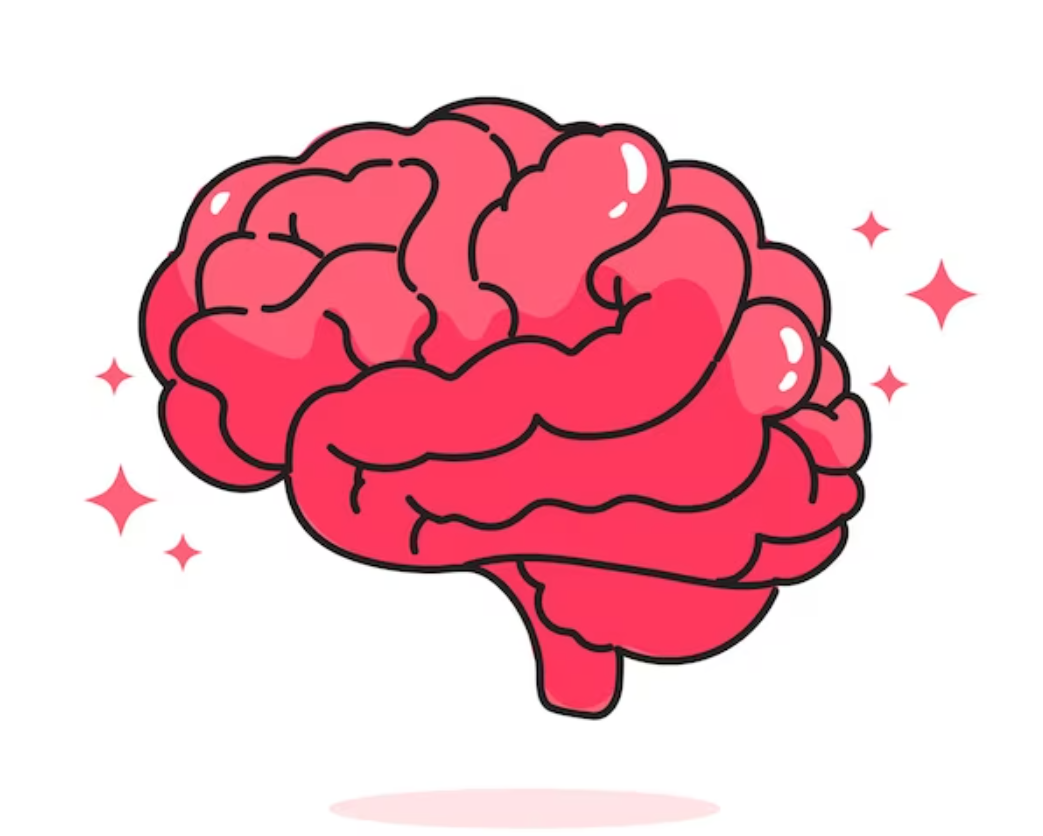
\includegraphics[width=\textwidth]{img/cerebro.png} % Asegúrate de cambiar la ruta a la ubicación de tu imagen
		\end{column}
		
		% Columna de la derecha
		\begin{column}{0.5\textwidth} % Ajusta la proporción según necesites
			\begin{itemize}
				\item Es el origen de pensamientos, sentimientos, decisiones y memorias.
				\item Coordina actividades como:
				\begin{itemize}
					\item Movimiento
					\item Visión
					\item Comunicación (oído, habla).
					\item Cantidad importante de \textit{\textbf{conexiones} entre neuronas.}
				\end{itemize}
			\end{itemize}
		\end{column}
	\end{columns}
\end{frame}

\begin{frame}
		\begin{center}
			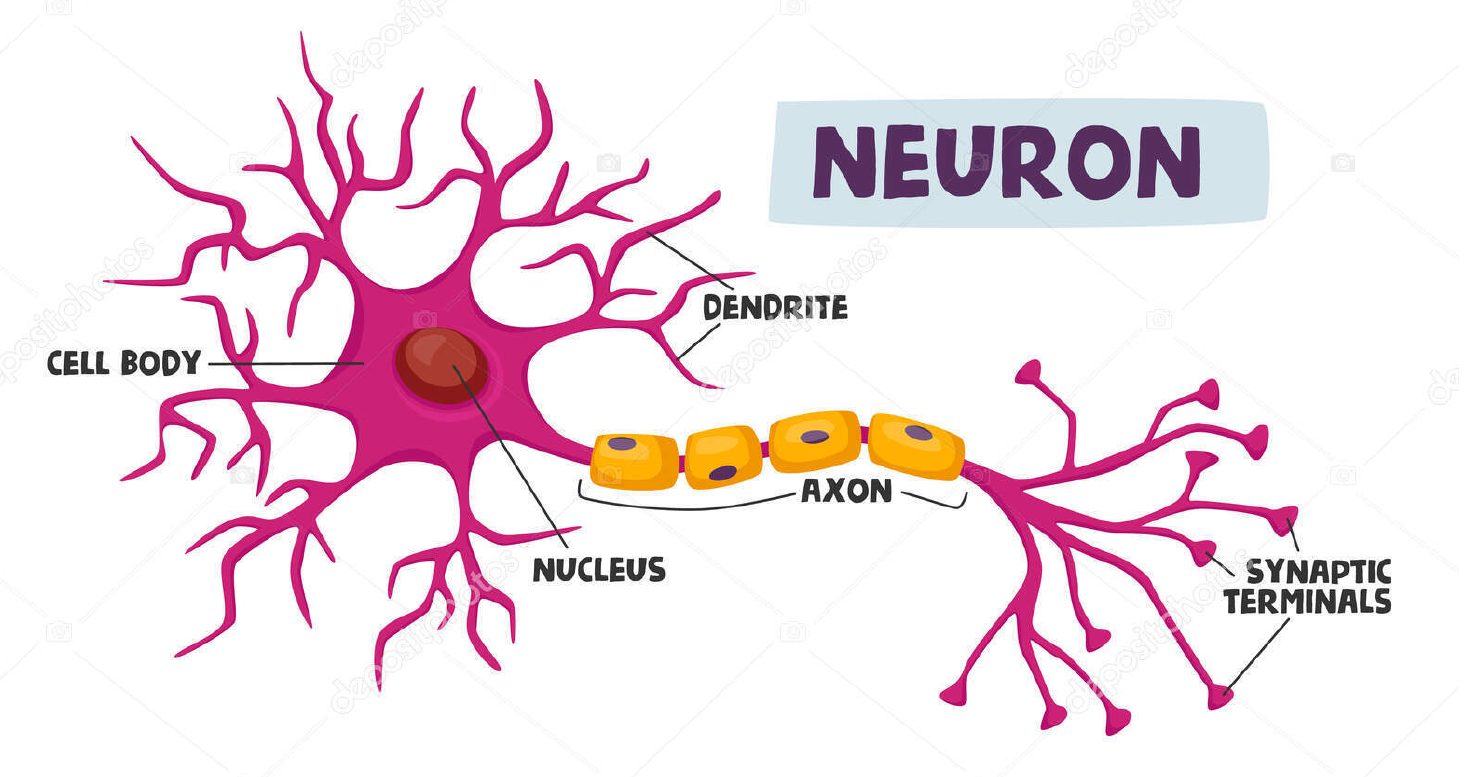
\includegraphics[width=12cm]{neurona.png}
		\end{center}
\end{frame}

%------------------------------------------------

\begin{frame}
	\frametitle{La Neurona Artificial}
	
	\begin{columns}
		
		% Columna de la izquierda
		\begin{column}{0.5\textwidth} % Ajusta la proporción según necesites
			
			De manera similar, la conexión (red) de neuronas artificiales, pueden \textbf{\textit{dotar a la máquina de}}:
			
			\begin{itemize}
				\item Coordinación para el movimiento.
				\item Visión artificial.
				\item Entendimiento del lenguaje natural.
				\item Habla.
				\item Comunicación.
				\item Reconocimiento de patrones.
				\item Capacidad de aprendizaje.
			\end{itemize}
			
		\end{column}
		
		% Columna de la derecha
		\begin{column}{0.5\textwidth} % Ajusta la proporción según necesites
			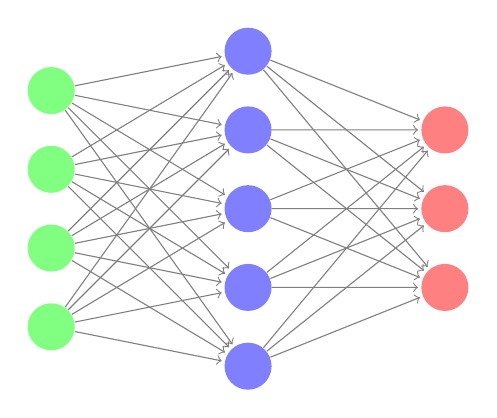
\begin{tikzpicture}[shorten >=1pt,->,draw=black!50, node distance=1cm]
				\tikzstyle{every pin edge}=[<-,shorten <=1pt]
				\tikzstyle{neuron}=[circle,fill=black!25,minimum size=17pt,inner sep=0pt]
				\tikzstyle{input neuron}=[neuron, fill=green!50];
				\tikzstyle{output neuron}=[neuron, fill=red!50];
				\tikzstyle{hidden neuron}=[neuron, fill=blue!50];
				\tikzstyle{annot} = [text width=4em, text centered]
				
				% Capa de entrada
				\foreach \name / \y in {1,...,4}
				\node[input neuron] (I-\name) at (0,-\y) {};
				
				% Capa oculta
				\foreach \name / \y in {1,...,5}
				\path[yshift=0.5cm]
				node[hidden neuron] (H-\name) at (2.5cm,-\y cm) {};
				
				% Capa de salida
				\foreach \name / \y in {1,...,3}
				\path[yshift=-0.5cm]
				node[output neuron] (O-\name) at (5cm,-\y cm) {};
				
				% Conexiones entrada-oculta
				\foreach \source in {1,...,4}
				\foreach \dest in {1,...,5}
				\path (I-\source) edge (H-\dest);
				
				% Conexiones oculta-salida
				\foreach \source in {1,...,5}
				\foreach \dest in {1,...,3}
				\path (H-\source) edge (O-\dest);
			\end{tikzpicture}
		\end{column}
		
	\end{columns}

\end{frame}


\begin{frame}
	\frametitle{Aplicaciones}
	\begin{columns}
		\begin{column}{0.25\textwidth}
			\centering
			
\includegraphics[width=\linewidth]{siri.jpg}
		\end{column}
		\begin{column}{0.25\textwidth}
			\centering
			
\includegraphics[width=\linewidth]{chat.jpg}
		\end{column}
		\begin{column}{0.25\textwidth}
			\centering
			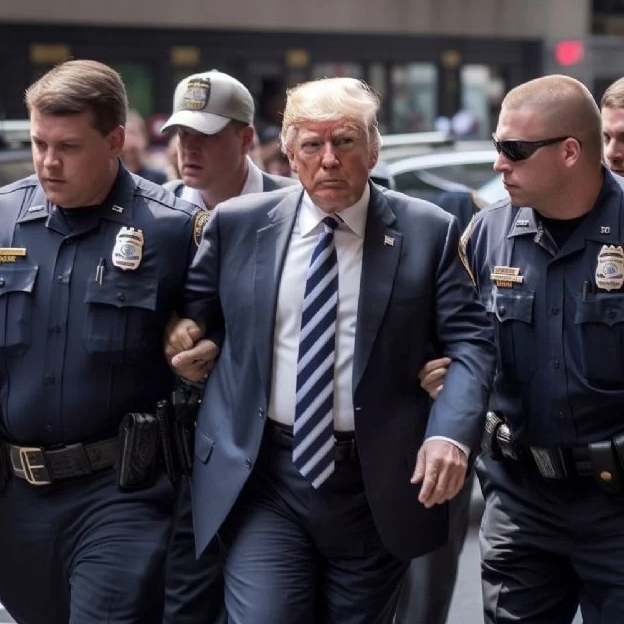
\includegraphics[width=\linewidth]{trump.png}
		\end{column}
		\begin{column}{0.25\textwidth}
			
\includegraphics[width=\linewidth]{maluma.jpeg}
		\end{column}
	\end{columns}
\end{frame}





%------------------------------------------------

